\documentclass[answers]{exam} % Clase para exámenes con respuestas
\usepackage[english,spanish]{babel} % Soporte para inglés y español
\usepackage[autostyle]{csquotes} % Manejo de citas
\usepackage{amsmath, amssymb} % Paquetes para matemáticas avanzadas
\usepackage{graphicx} % Inclusión de gráficos
\usepackage{wrapfig}
\usepackage{enumitem} % Personalización de listas enumeradas
\usepackage[letterpaper,top=2cm,bottom=2cm,left=3cm,right=3cm,marginparwidth=1.75cm]{geometry} % Configuración de márgenes
\usepackage[colorlinks=true, allcolors=blue]{hyperref} % Enlaces con color

\usepackage{array}   % for adjusting row height
\renewcommand{\arraystretch}{1.5} % adjust the vertical spacing between rows

\renewcommand{\solutiontitle}{\noindent\textbf{Respuesta:}\par\noindent} % Personalización del título de respuestas
\renewcommand{\familydefault}{\sfdefault}

% Configuración de encabezado y pie de página
\pagestyle{headandfoot}
\firstpageheader{Universidad de Bolívar}{}{Noviembre 19, 2024} 
\runningheader{Universidad de Bolívar}{}{Física}
\firstpagefooter{}{\thepage}{}
\runningfooter{}{\thepage}{}

\begin{document}

\begin{center}
	\large\textbf{Trabajo Autónomo 2.11 - Fundamentos de Física para Ingeniería}\\[1em]
	\large Segundo Ciclo \enquote*{A} - Ingeniería de Software\\[1em]
\end{center}

\vspace{0.5cm}
\noindent
\large\textbf{Tema:} DIAELÉCTRICOS Y CONDENSADORES \\
\large\textbf{Estudiante:} Ariel Alejandro Calderón
\vspace{0.5cm}

\begin{questions}

	% Question 1
	\question \large\textbf{Presentar una tabla con las fórmulas de las derivadas de las funciones básicas:}
	\begin{center}
		\begin{wrapfigure}{l}{1\textwidth}
			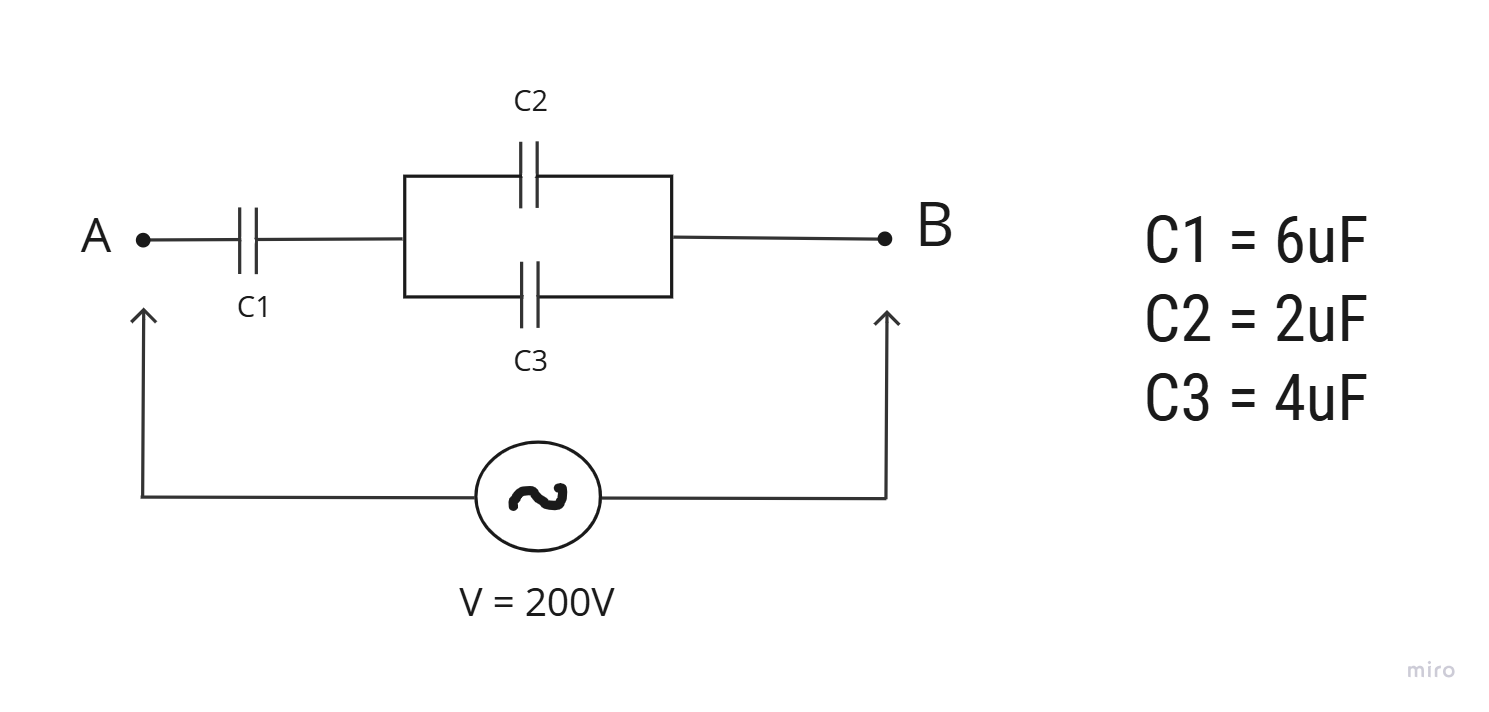
\includegraphics[width=1\textwidth]{./public/g1.png}
		\end{wrapfigure}
	\end{center}

	\vspace{0.5cm}
\end{questions}

\end{document}